\begin{enumerate}
\item[1.]
\begin{figure}[ht]
    \centering
    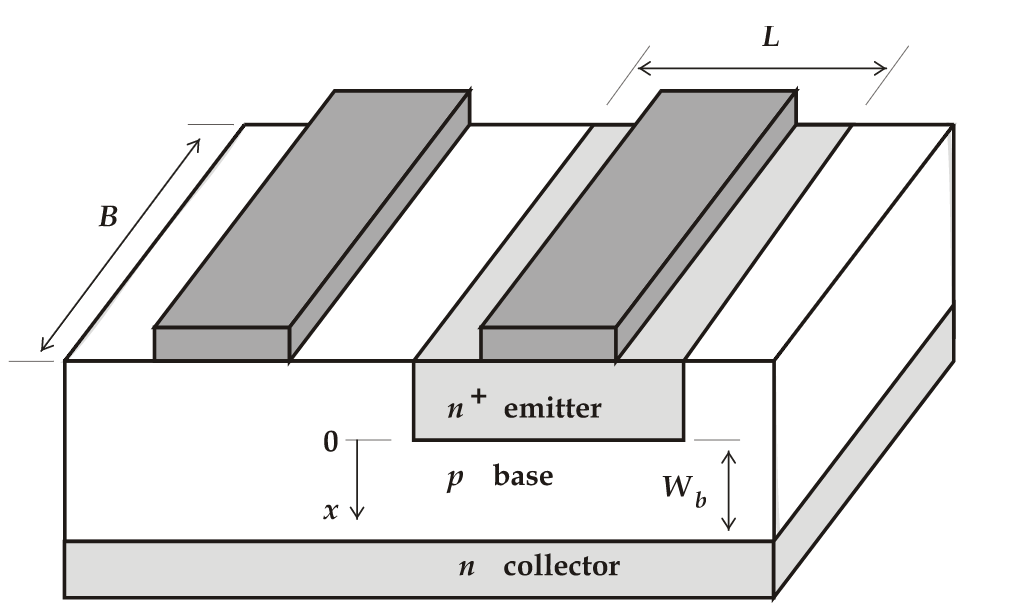
\includegraphics[width=\linewidth]{figures/simple_transistor.PNG}
    \caption{Figure 4 from the lab manual of a simple transistor}
    \label{fig:transitor}
\end{figure}
The figure above is that of a simple transistor from the lab manual. The formula for $I_{CS}$ is:
\begin{equation}
    I_{CS} = \frac{q A_e n_i^2 D_n}{N_{Ab}W_b}
\end{equation}
so if you increase $W_b$ then you are going to lower the gain $\beta_F = \frac{I_C}{I_B}$, but it will increase the switching time


\item[2.]
The three types of materials are:
\begin{labeling}[:]{N\texttt{+} type}
\item [N\texttt{+} type] a n-type semiconductor with a high, often degenerate doping concentration.
\item [N type] a semiconductor that having more conduction electrons than mobile holes.
\item [P type]  a semiconductor having a density of mobile holes in excess of that of conduction electrons.
\end{labeling}


\item[3.]
The four transistor operation modes are:
\begin{labeling}{Reverse-Active}
\item [Saturation] The transistor acts like a short circuit. Current freely flows from collector to emitter.
\item [Cut-off] The transistor acts like an open circuit. No current flows from collector to emitter.
\item [Active] The current from collector to emitter is proportional to the current flowing into the base.
\item [Reverse-Active] Like active mode, the current is proportional to the base current, but it flows in reverse. Current flows from emitter to collector (not, exactly, the purpose transistors were designed for).
\end{labeling}

\item[5.]
The current gain $\beta$ is theoretically constant, but as the question states at high and low values of $I_C$ we see that the the gain decreases. This is due to leakage mechanism in the transistor for low $I_C$ and  due to high level injection for high $I_C$.
\item[6.]
\begin{labeling}{Gummel Plot}
\item [Gummel Plot] A plot which shows $I_C$ versus $V_{BE}$ characteristics of a transistor, this is completed on a semi-log plot where the current is on the log scale.
\item [I\textsubscript{CS}] The collector saturation current is where the base current so that the emitter-base junction is forward biased. In fact, the base current has increased beyond the point where it can cause the collector current flow to increase. At this point, collector emittor currents have increased to a maximal value.
\item [D\textsubscript{n av}] D\textsubscript{n} is the electron diffusion coefficient in the base, which is a physical constant which describing how electrons move through the p-type base. The D\textsubscript{n av} is simply the average of this value throughout the material.
\end{labeling}

\item[7.] The reason that the current gain $\beta \left( \frac{I_C}{I_B} \right) $ decreases at low values of $I_C$ is clear, the ideal model of gain which is shown by $\beta  = \frac{I_C}{I_B}$ is accurate, and hence  $I_C \propto \beta$.

However the reason that the current gain decreases at high values of $I_C$ is not as simple, we deviate from the ideal line equation due to the base resistance and emitter  resistance of the transistor. These resistances are only relevant at high currents as they are non-idealities.

%This is caused because the Voltage ($V_{BE}$) is maintained at a constant value, but when the currents through the device become large the resistances of the emittor and base become significant. This is modelled through the equation: $V_{BE eff} = V_{BE} - \frac{I_{C}}{\beta} r_{bb} - \frac{I_{C}(\beta - 1)}{\beta} r_e$ where $r_e$ and $r_{bb}$ are the emittor and base resistance respectively. There are also other high current effects that come into play


\item[8.]
The differences between the different types of resistors are:
\begin{labeling}{P type pinched resistor}
\item [P type pinched resistor] is a n type region surrounded by a thin p region, known as the pinching region, which is again covered by a n region. It works by lowering the crossectional area and only allowing a small reverse current. These types of resistors can have very high resistances but are often more difficult to manufacture.
\item [P type resistor] is a formed in any one of the isolated regions of p doping, surrounded by a n-region. The differences in resistance are generally controlled by the doping and then crossectional area can also be controlled, but is much larger than the pinched resistors as we only have two layers. 
\item [Carbon resistor] is not a solid state resistor and is not created by using deposition. These different resistance values are generated by varying the length of resistive material that the electricity passes through. This resistive material is made of graphite, ceramic dust and resin.
\end{labeling}

\item[9.]

We see here that the figure below has both the pinched and non-pinched p-type resistor. We know that the calculation of the cross-sectional area will be height times thickness of the resistive material. We note that in our figures, the height will be consistant between both the pinched and unpinched resistor, however the thickness will not be. The thickness of the p-type material will be $t_p$, but the thickness of the pinched resistor will be $t_p - t_n$, since it is deposited above it. This difference in thicness will decrease the area, and effectively increase the resistance.


\begin{figure}[h]
    \begin{subfigure}[b]{\linewidth}
    \centering
    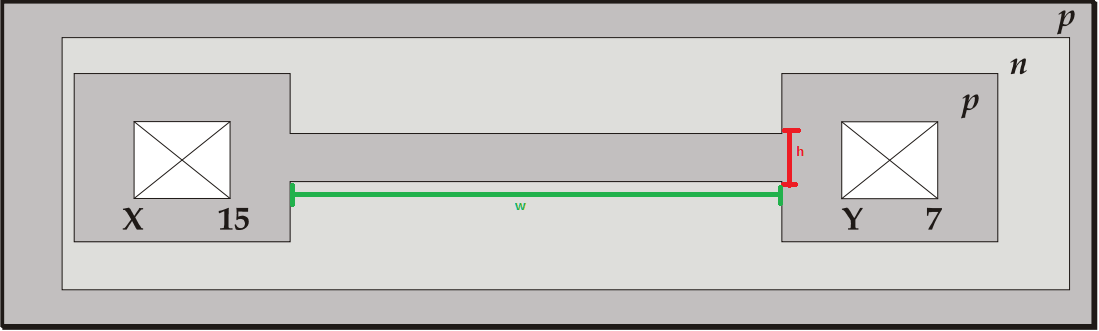
\includegraphics[width=0.95\linewidth]{figures/p_resist.png}
    \caption{Top down diagram of a p-type resistor}
    \label{fig:p_resist}
    \end{subfigure}
    \begin{subfigure}[b]{\linewidth}
    \centering
    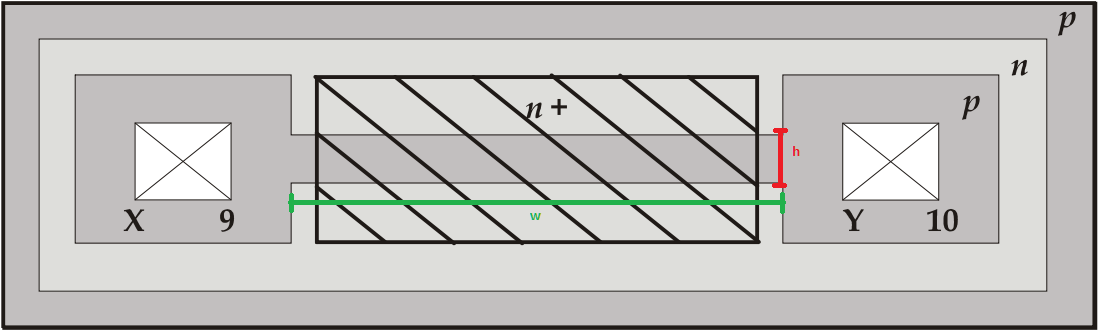
\includegraphics[width=0.95\linewidth]{figures/p_pinched_resist.png}
    \caption{Top down diagram of a p-type pinched resistor}
    \label{fig:pinched_resist}
    \end{subfigure}
\end{figure}

\end{enumerate}
